\begin{center}
	\LARGE Delprøve uden hjælpemidler (12:10 - 13:25)
\end{center}
\begin{opgavetekst}{Opgave 1}
	På Figur \ref{fig:vektorer} kan vi se to vektorer $\vv{a}$ og $\vv{b}$ samt et skraveret område $M$.
	\begin{figure}[H]
		\centering
		\begin{tikzpicture}
			\begin{axis}[
				axis lines = center, 
				xmin = -1.5, xmax = 7.5, 
				ymin = -1.5, ymax = 7.5, 
				x = 1.0cm, y = 1.0cm,
				grid,
				xlabel = $x$, ylabel = $y$
			]
				\draw[-{Stealth[scale=1.5]}, thick, color = teal] (axis cs: 1,5) -- (axis cs: 5,7) node[midway, xshift = -7pt, yshift = 7pt] {$\vv{a}$};
				\draw[-{Stealth[scale=1.5]}, thick, color = teal] (axis cs: 1,5) -- (axis cs: 3,2) node[midway, xshift = 7pt, yshift = 7pt] {$\vv{b}$};
				\fill[olive,nearly transparent] (axis cs: 1,5) -- (axis cs: 5,7) -- (axis cs:7,4) -- (axis cs: 3,2) -- cycle;
				\node[color = teal] at (axis cs: 4,4.5) {$M$};
			\end{axis}
		\end{tikzpicture}
		\caption{To vektorer.}
		\label{fig:vektorer}
	\end{figure}
	\phantom{h}
\end{opgavetekst}
\begin{delopgave}{(10 point)}{1}
	Afgør, om vektorerne $\vv{a}$ og $\vv{b}$ er orthogonale.
\end{delopgave}
\begin{delopgave}{(10 point)}{2}
	Bestem arealet af det skraverede område $M$. 
\end{delopgave}


\begin{opgavetekst}{Opgave 2}
	To funktioner $f$ og $g$ er givet ved
	\begin{align*}
		f(x) = \sqrt{x}
	\end{align*}
	og 
	\begin{align*}
		g(x) = x^4-2x^2-4.
	\end{align*}
\end{opgavetekst}
\begin{delopgave}{(10 point)}{1}
	Bestem $f(g(2))$.
\end{delopgave}

\begin{opgavetekst}{Opgave 3}
	På Figur \ref{fig:parabel} ses parablen for andengradspolynomiet $f$ givet ved
	\begin{align*}
		f(x) = ax^2+bx+c
	\end{align*}
	
	\begin{figure}[H]
		\centering
		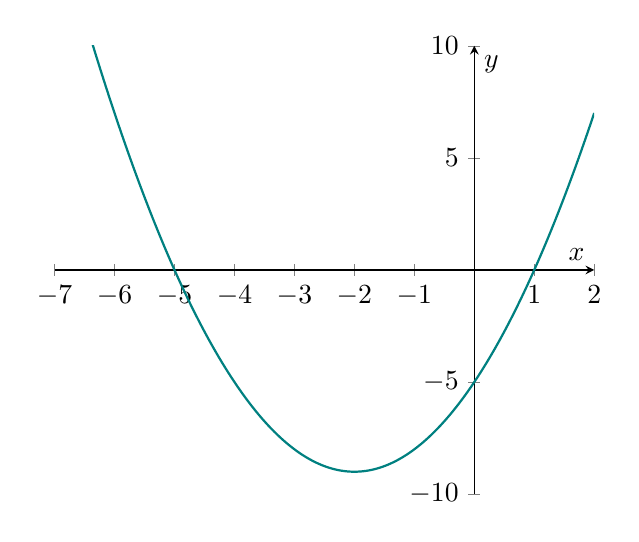
\begin{tikzpicture}
			\begin{axis}[
			axis lines = middle, 
			xmin = -7, xmax = 2,
			ymin = -10, ymax = 10,
			xtick = {-7,-6,...,4,5},
			ytick = {},
			xlabel = $x$, ylabel = $y$,
			]
				\addplot[color = teal, samples = 200, thick, domain = -7:2] {(x+5)*(x-1)};
			\end{axis}
		\end{tikzpicture}
		\caption{Parabel for andengradspolynomiet $f$.}
		\label{fig:parabel}
	\end{figure}
	\phantom{h}
\end{opgavetekst}
\begin{delopgave}{(10 point)}{1}
	Bestem tallet $c$ og afgør, om tallene $a$ og $b$ er større eller mindre end $0$.
\end{delopgave}
\begin{delopgave}{(5 point)}{2}
	Aflæs rødderne for $f$. 
\end{delopgave}


	

\newpage

\begin{opgavetekst}{Opgave 4}
	Grafen for en eksponentialfunktion $g$ kan ses på Figur \ref{fig:exp}
	\begin{figure}[H]
		\centering
		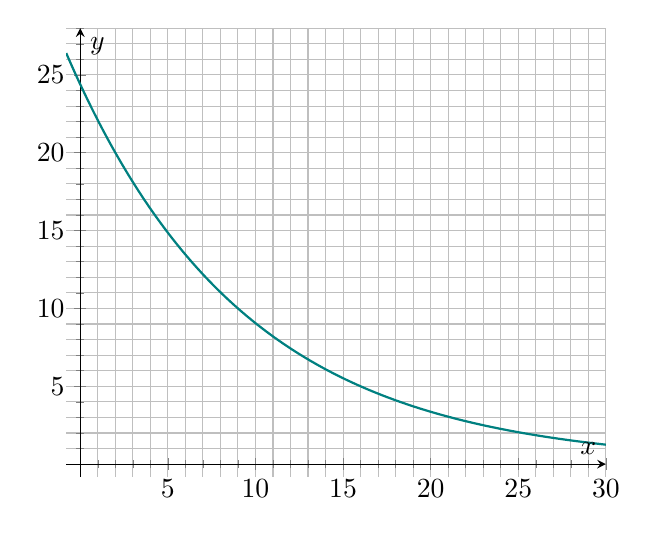
\begin{tikzpicture}
			\begin{axis}[
				axis lines = center,
				xmin = -0.8, xmax = 30,
				ymin = -0.8,ymax = 28,
				grid = both,
				minor tick num = 4,
				xlabel = $x$, ylabel = $y$
			]
				\addplot[thick, samples = 1000, color = teal, domain = -0.8:40] {24.390*0.90572^x};
			\end{axis}
		\end{tikzpicture}
		\caption{Grafen for eksponentialfunktionen $g$.}
		\label{fig:exp}
	\end{figure}
	\phantom{h}
\end{opgavetekst}
\begin{delopgave}{(10 point)}{1}
	Aflæs halveringskonstanten for $g$. Brug det vedlagte bilag. 
\end{delopgave}

\begin{opgavetekst}{Opgave 5}
	Et andengradspolynomium $p$ er givet ved forskriften
	\begin{align*}
		p(x) = 2x^2 - 4x - 6.
	\end{align*}
\end{opgavetekst}
\begin{delopgave}{(10 point)}{1}
	Bestem rødderne for $f$. 
\end{delopgave}


\newpage
\begin{center}
	\LARGE Delprøve med hjælpemidler (13:25 - 15:10)
\end{center}

\begin{opgavetekst}{Opgave 6}
	\begin{center}
		\includegraphics[width = 0.6\textwidth]{Billeder/proxima_centauri_b}
	\end{center}
	En gruppe mennesker har i en fjern fremtid besluttet sig for, at de vil kolonisere exoplaneten Proxima Centauri b. De rejser 1423 personer afsted, og de forventer, at 
	deres befolkningsudvikling kan beskrives ved eksponentialfunkionen $f$ givet ved
	\begin{align*}
		f(t) = 1423 \cdot 1.02^t,
	\end{align*}
	hvor $t$ betegner den forløbne tid siden ankomsten til planeten i jord-år, og $f$ betegner størrelsen på kolonien i antal personer. 
\end{opgavetekst}
\begin{delopgave}{(10 point)}{1}
	Bestem antallet af mennesker, de vil forvente at være i kolonien efter 50 år.
\end{delopgave}
\begin{delopgave}{(10 point)}{2}
	Afgør, hvor længe der vil gå, før kolonien vil være fordoblet i størrelse.
\end{delopgave}

\begin{opgavetekst}{Opgave 7}
	\begin{center}
		\includegraphics[width = 0.6\textwidth]{Billeder/slik}
	\end{center}
	En gruppe gymnasieelever har målt diameteren af forskellige stykker nogenlunde runde stykker slik og har derefter vejet dem. De forventer, at sammenhængen mellem slikkets 
	diameter $x$ i mm og vægten af slikket $g$ i gram kan beskrives ved en sammenhæng af typen
	\begin{align*}
		g(x) = b \cdot x^a.
	\end{align*}	 
	Resultatet af deres dataindsamling kan findes \href{https://github.com/ChristianJLex/TeachingNotes/raw/master/2023-2024/Data%20og%20lign/Slikvaegt.xlsx}{\color{blue!60} her.}
\end{opgavetekst}
\begin{delopgave}{(10 point)}{1}
	Brug datasættet til at bestemme tallene $a$ og $b$.
\end{delopgave}
\begin{delopgave}{(10 point)}{2}
	Bestem vægten af et stykke slik med en diameter på 20mm.
\end{delopgave}
\begin{meretekst}
	Bent påstår, at han kan spise et stykke slik på 100g i én mundfuld. De andre udviser en vis skepsis og beder derfor Bent om at åbne munden, så de kan 
	måle, hvor stor afstanden fra hans tænder er. De måler afstanden til at være 30mm. 
\end{meretekst}
\begin{delopgave}{(10 point)}{3}
	Afgør, om Bent rent faktisk kan gabe over et stykke slik på 100g. 
\end{delopgave}

\begin{opgavetekst}{Opgave 8}
	To vektorer $\vv{a}$ og $\vv{b}$ er givet ved
	\begin{align*}
		&\vv{a} = 
		\begin{pmatrix}
			t^3 \\ -4		
		\end{pmatrix}
		& 
		&\textnormal{og}
		&
		&\vv{b} =
		\begin{pmatrix}
			t-4 \\ t^2
		\end{pmatrix}
	\end{align*}
\end{opgavetekst}
\begin{delopgave}{(10 point)}{1}
	Bestem prikproduktet mellem $\vv{a}$ og $\vv{b}$, hvis $t = -7$. 
\end{delopgave}
\begin{delopgave}{(10 point)}{2}
	Bestem den værdi for $t$, der gør $\vv{a}$ og $\vv{b}$ parallelle. 
\end{delopgave}

\begin{opgavetekst}{Opgave 9}
	\begin{center}
		\includegraphics[width = 0.6\textwidth]{Billeder/Fjordenhus}
	\end{center}
	I Vejle ligger Fjordenhus, der som en del af facaden har parabellignende buer. Én af buerne kan ses indlejret i et koordinatsystem på Figur \ref{fig:fjordenhus}.
	\begin{figure}[H]
		\centering
		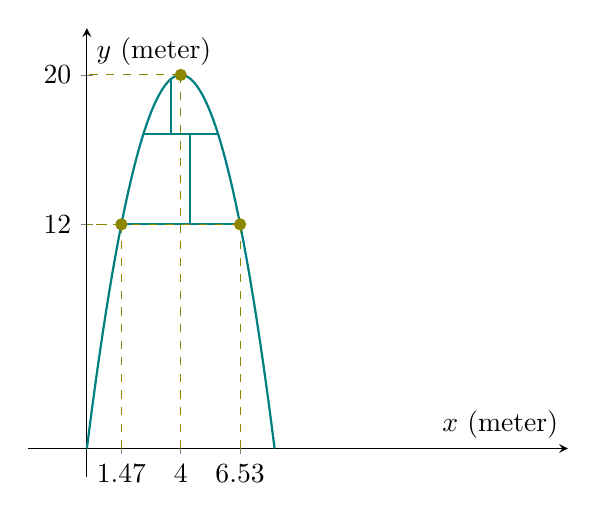
\begin{tikzpicture}
			\begin{axis}[
				axis lines = middle, 
				xmin = -2.5, 
				xmax = 20.5,
				ymin = -1.5,
				ymax = 22.5,
				xlabel = {$x$ (meter)},
				ylabel = {$y$ (meter)},
				xtick = {1.47,4,6.53},
				ytick = {12,20}
			]
				\addplot[color = teal, thick, samples = 150, domain = 0:8] {-1.25*x^2+10*x};
				\draw[color = teal, thick] (axis cs: 1.47,12) -- (axis cs: 6.53,12);
				\draw[color = teal, thick] (axis cs: 2.41,16.84) -- (axis cs: 5.59,16.84);
				\draw[color = teal, thick] (axis cs: 3.6,19.8) -- (axis cs: 3.6,16.84);
				\draw[color = teal, thick] (axis cs: 4.4,16.84) -- (axis cs: 4.4,12);
				\filldraw[color = olive] (axis cs: 1.47,12) circle (2pt);
				\filldraw[color = olive] (axis cs: 6.53,12) circle (2pt);
				\filldraw[color = olive] (axis cs: 4,20) circle (2pt);
				\draw[color = olive, dashed] (axis cs: 1.47,0) -- (axis cs: 1.47,12);
				\draw[color = olive, dashed] (axis cs: 1.47,12) -- (axis cs: 0,12);
				\draw[color = olive, dashed] (axis cs: 6.53,12) -- (axis cs: 0,12);
				\draw[color = olive, dashed] (axis cs: 6.53,12) -- (axis cs: 6.53,0);
				\draw[color = olive, dashed] (axis cs: 4,0) -- (axis cs: 4,20);
				\draw[color = olive, dashed] (axis cs: 4,20) -- (axis cs: 0,20);
			\end{axis}
		\end{tikzpicture}
		\caption{Skitse af facadeparabel på Fjordenhus.}
		\label{fig:fjordenhus}
	\end{figure}
	\phantom{h}
\end{opgavetekst}
\begin{delopgave}{(10 point)}{1}
	Bestem en forskrift for den parabel, der fremgår af Figur \ref{fig:fjordenhus}.
\end{delopgave}
\begin{delopgave}{(5 point)}{2}
	Afgør, hvor bred facadebuen på Fjordenhus er i vandoverfladen. 
\end{delopgave}
\newpage
\phantom{h}
\newpage
\begin{center}
	\LARGE Bilag:
\end{center}
\begin{center}
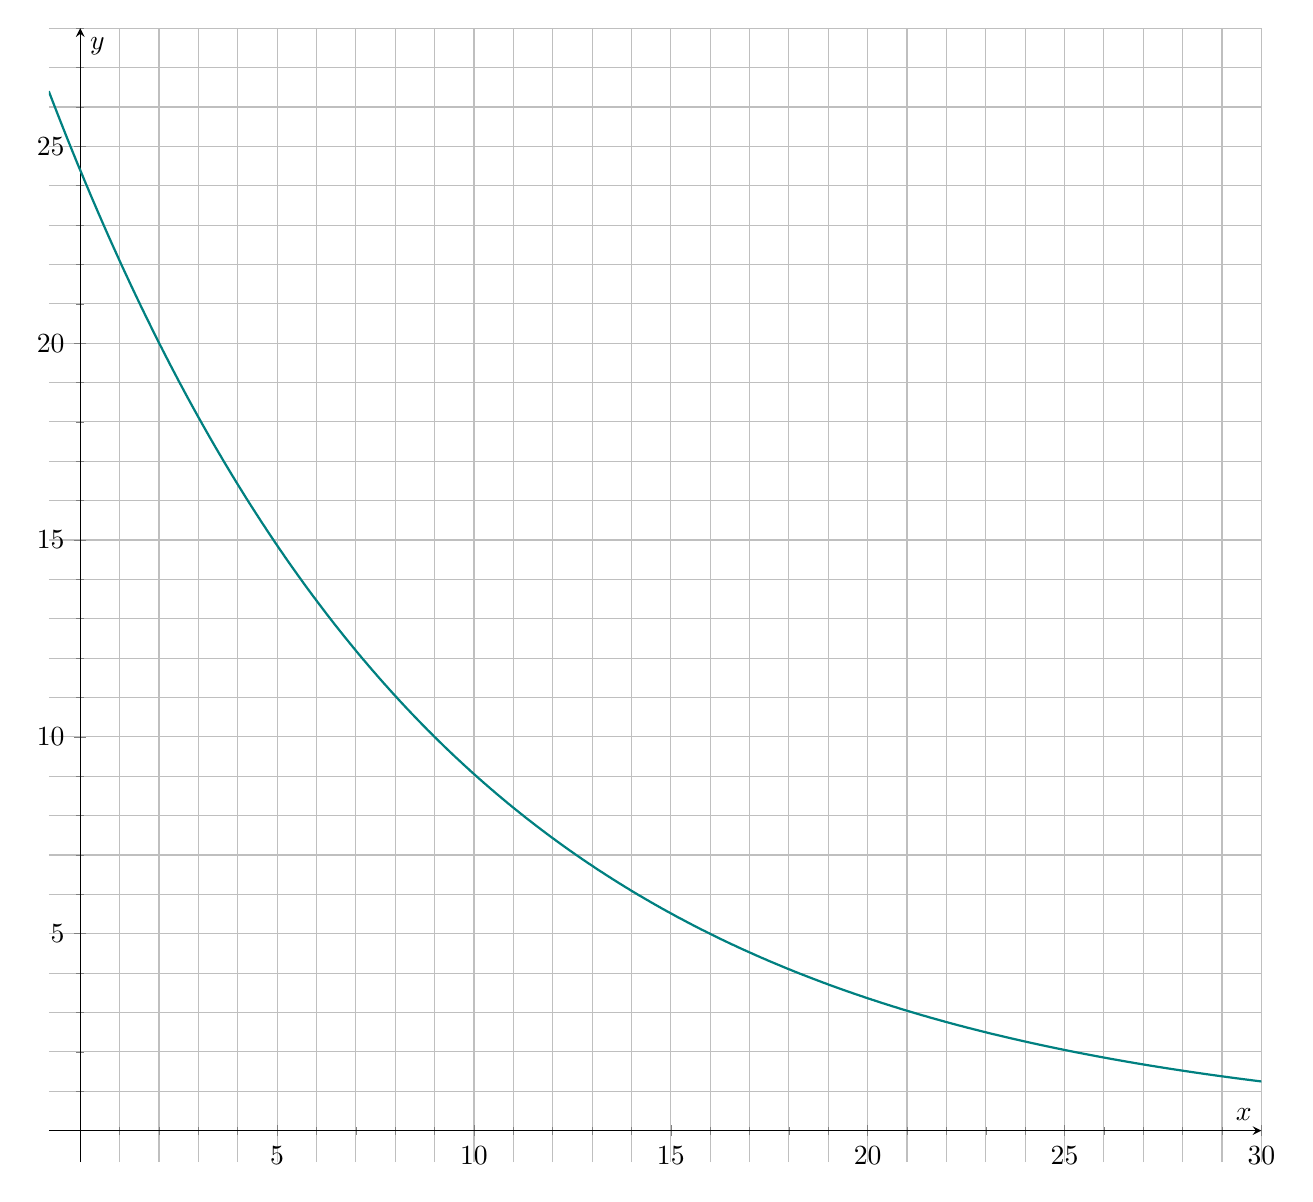
\begin{tikzpicture}
			\begin{axis}[
				axis lines = center,
				xmin = -0.8, xmax = 30,
				ymin = -0.8,ymax = 28,
				grid = both,
				xtick = {0,5,...,25,30},
				ytick = {0,5,...,25,30},
				minor tick num = 4,
				xlabel = $x$, ylabel = $y$,
				x = 0.5cm, y = 0.5cm
			]
				\addplot[thick, samples = 1000, color = teal, domain = -0.8:40] {24.390*0.90572^x};
			\end{axis}
		\end{tikzpicture}
\end{center}
Bilaget vedlægges, når du afleverer Delprøve 1.
